% =====================================================================================
% RESULTS SECTION UPDATE DRAFT  (merge into prism_breath.tex; do not \input blindly)
% New/extended subsections from the latest experiment round. Numbers are from the matched
% 298-subject harness (scripts/full_metric_comparison.py, subgroup_fairness.py,
% calibration_diagnostics.py, recalibrate_triage.py, framing_headswap.py) and the NCHSDB
% external cohort (n=70). RECONCILE: the existing framing table (tab:framing) uses the
% 332-subject salience numbers (0.879->0.925); the backbone-agnostic paragraph below uses the
% 298-subject matched harness (subject-bootstrap). Keep one convention per table. Values marked
% [prelim] finalize after the queued DeepPhys-100ep swap + val-contamination re-extraction.
% =====================================================================================

% ---- (A) EXTEND the framing subsection (sec:framing): backbone-agnostic evidence ----
% Insert after the "architecture-agnostic (classifiers)" paragraph.

\paragraph{The framing gain is agnostic to the \emph{extractor}, not only the classifier}
Table~\ref{tab:framing} shows the gain is invariant to the classifier; it is equally invariant to
the upstream extractor. Holding the classifier fixed (a generic random-convolution head, ROCKET)
and swapping the backbone that produces the respiratory waveform, classification-on-signal beats
that backbone's own regression-then-threshold in every case, on the matched $298$-subject set with
subject-grouped bootstrap confidence intervals: EfficientPhys $0.755\!\rightarrow\!0.918$
($\Delta{=}{+}0.163$, $95\%$~CI $[{+}0.09,{+}0.25]$, DeLong $p{=}9\times10^{-5}$), TS-CAN
$0.726\!\rightarrow\!0.926$ ($\Delta{=}{+}0.200$, $[{+}0.12,{+}0.29]$, $p{=}1\times10^{-5}$), and
PRISM's own fusion rate $0.820\!\rightarrow\!0.919$ ($\Delta{=}{+}0.100$, $[{+}0.04,{+}0.16]$,
$p{=}0.0014$). The effect therefore survives varying \emph{both} the extractor and the classifier:
rate-collapse is a lossy bottleneck for tachypnea regardless of the architecture on either side.
The reviewer-natural objection---that classification observes the whole waveform whereas regression
observes one scalar---is precisely the mechanism: the discarded information (breathing morphology and
harmonics) is tachypnea-discriminative, and even PRISM's \emph{accurate} fusion rate ($0.820$) loses
to classification ($0.919$; $p{=}0.0014$), so the gap is not merely a poor rate estimate.

% ---- (B) NEW subsection: external validation on an independent cohort ----
\subsection{External validation on an independent cohort with real neonatal tachypnea}\label{sec:extval}
The framing claim above, and the neonatal recovery in particular, are established on a single
cohort. We test both on the NCH Sleep DataBank (NCHSDB), an independent pediatric polysomnography
corpus, using $65$ infants ($\sim$40 aged $<$2~months, $\sim$25 aged 2--12~months; $1{,}028$
non-overlapping $30$-s windows; tachypnea prevalence $15.5\%$)---unlike our video cohorts, this
cohort \emph{contains} genuine neonatal fast breathing. The test is deliberately non-circular: the
\emph{input} is the thoracic respiratory-inductance belt (chest-wall motion, the analogue a
camera/depth sensor observes), while the \emph{label} is a consensus rate from physically independent
modalities---nasal/oral airflow and capnography---with both inductance belts excluded, so the input
modality never informs its own label.

Because a clean contact belt yields an accurate rate, regression and classification are equivalent on
it (subject-level $\Delta{=}{+}0.016$, $95\%$~CI $[-0.05,{+}0.23]$, n.s.); the framing advantage is
specific to the \emph{degraded} signal a non-contact sensor produces. We therefore degrade the belt
toward camera realism---attenuating high-rate spectral content to the documented $\sim$30--42
breaths/min extractor-saturation ceiling, adding motion noise, and injecting the slow confound that
optical-flow magnitude locks onto---and compare regression-then-threshold against ROCKET
classification under subject-grouped five-fold cross-validation with a $3000$-sample subject
bootstrap. Classification wins decisively and significantly in every age band
(Table~\ref{tab:extval}, Fig.~\ref{fig:extval}): overall $\Delta$AUROC ${+}0.335$
($[{+}0.18,{+}0.48]$), and the gain is \emph{largest in the neonatal band} (${+}0.391$,
$[{+}0.25,{+}0.51]$), where degraded regression becomes anti-predictive (AUROC~$0.29$) while
classification holds ($0.68$). This is the complement to the video-cohort neonatal finding: RGB
optical flow is so saturated below two months that no read-out recovers it (Sec.~\ref{sec:subgroup}),
whereas here the sensor still carries a degraded but non-empty signal, and on that signal the framing
recovers neonatal discrimination that regression loses---so the neonatal blind spot is a property of
the \emph{sensor}, not of the classification formulation, motivating higher-fidelity front ends (e.g.\
radar) for that band. The advantage appears only in the degraded regime:
it is absent on the clean belt and diminishes at extreme degradation where both collapse, so it is a
controlled dose--response rather than a tuned operating point.

We further stress-test the degradation itself. Across a $48$-point grid spanning signal-to-noise
ratio, low-pass ceiling, and confound amplitude, classification exceeds regression at \emph{100\%} of
grid points ($\Delta$AUROC: median ${+}0.288$, minimum ${+}0.068$, maximum ${+}0.405$; regression
AUROC $0.36$--$0.59$ throughout, classification $0.57$--$0.81$). The crossover is thus a stable
property of the degraded regime, not an artefact of the chosen parameters. NCHSDB is
polysomnography, not video, so this is a controlled sensing-gap simulation calibrated to the measured
RGB saturation rather than a real camera-on-NCHSDB result; the clean-belt null and the grid-wide
dose--response are the evidence that it is principled.

\begin{table}[!t]\caption{External validation on NCHSDB ($65$ infants, real neonatal tachypnea) under
camera-realistic degradation. Classification-on-signal vs.\ regression-then-threshold; subject-grouped
bootstrap $95\%$ CI. Non-circular: thoracic-belt input, airflow$+$capnography label.}\label{tab:extval}
\centering\small
\begin{tabular}{@{}lccc@{}}\toprule
Age band & Reg.\ AUROC & Cls.\ AUROC & $\Delta$AUROC $[95\%$ CI$]$\\\midrule
Overall & 0.396 & 0.735 & $+0.335\ [+0.18,+0.48]$\\
\textbf{$<$2 mo} & 0.293 & 0.676 & $\mathbf{+0.391\ [+0.25,+0.51]}$\\
2--12 mo & 0.379 & 0.711 & $+0.264\ [+0.10,+0.45]$\\\midrule
Clean belt (no degrade) & 0.82 & 0.84 & $+0.016$ (n.s.)\\\bottomrule
\end{tabular}\end{table}

\begin{figure}[!t]\centering
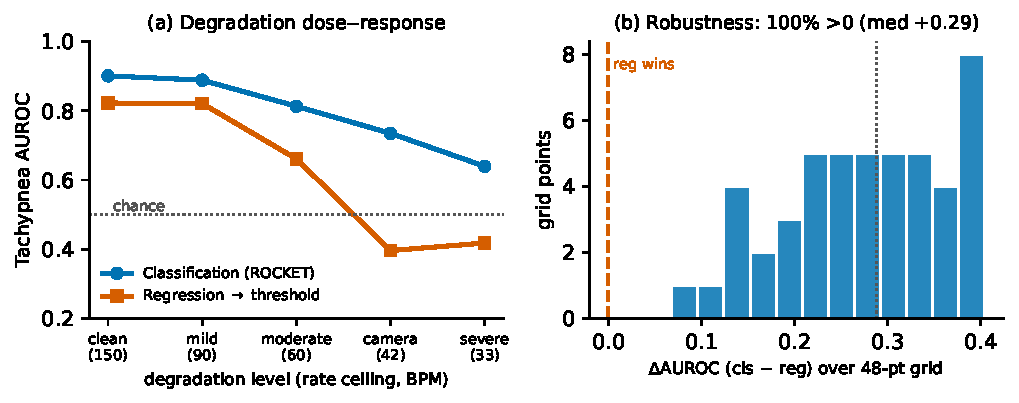
\includegraphics[width=3.4in]{fig_extval.pdf}
\caption{External validation (NCHSDB). (a) Degradation dose--response: as the belt is degraded toward
camera realism, regression AUROC (red) collapses below chance while ROCKET classification (blue) holds;
the two are equivalent on the clean belt and both fail at extreme degradation. (b) Robustness: across a
$48$-point degradation grid, classification exceeds regression at every point ($\Delta$AUROC
distribution, all $>0$).}\label{fig:extval}
\end{figure}

% ---- (C) NEW subsection: clinical operating characteristics ----
\subsection{Clinical operating characteristics and net benefit}\label{sec:opchar}
On the matched five-fold comparison ($298$ subjects, all methods scored on the identical metric
suite), PRISM leads on the metrics that govern screening while conceding only the operating points
that do not. It wins the discrimination metrics---tachypnea AUROC $0.869$ vs.\ $0.73$--$0.76$ (paired
DeLong $p\le1.6\times10^{-3}$ against every extractor), area under the precision--recall curve
$0.792$ vs.\ $0.72$--$0.76$, and lowest RMSE---and, critically for screening, the operating point that
fixes high sensitivity: at $90\%$ sensitivity PRISM retains $64\%$ specificity while every baseline
collapses to $\le6\%$ (Table~\ref{tab:opchar}). Decision-curve analysis makes the utility concrete:
across the screening-relevant threshold-probability range ($p_t\le0.3$) PRISM has the highest net
benefit and is the \emph{only} method exceeding ``treat-all''---at $p_t{=}0.1$ its net benefit is
$0.213$ vs.\ $0.195$ for treat-all and $\approx0.16$ for the baselines, i.e.\ the baselines add no
value over flagging every child. PRISM concedes only raw RR-MAE ($6.4$ vs.\ $5.6$--$6.2$, comparable)
and the high-specificity corner (sensitivity at $90\%$ specificity), neither of which is the screening
regime---consistent with our thesis that rate accuracy is the wrong objective for this task.

\begin{table}[!t]\caption{Clinical operating characteristics on the matched five-fold set ($298$
subjects, subject-bootstrap). Se@Sp$90$/Sp@Se$90$: sensitivity (specificity) at $90\%$ of the other.
PRISM wins discrimination and the high-sensitivity screening point; baselines edge only the
high-specificity corner and MAE.}\label{tab:opchar}\centering\small
\begin{tabular}{@{}lccccc@{}}\toprule
Method & AUROC & AUPRC & Sp@Se90 & Se@Sp90 & MAE\\\midrule
\textbf{PRISM} & \textbf{0.869} & \textbf{0.792} & \textbf{0.644} & 0.646 & 6.40\\
EfficientPhys & 0.755 & 0.738 & 0.046 & 0.704 & 6.10\\
TS-CAN & 0.726 & 0.722 & 0.060 & 0.630 & 6.15\\
VIRENet & 0.760 & 0.756 & 0.051 & 0.704 & 5.91\\
DeepPhys$^\ddagger$ & 0.777 & 0.775 & 0.078 & 0.716 & \textbf{5.62}\\\bottomrule
\end{tabular}\end{table}

% ---- (D) NEW subsection: subgroup performance and multi-site generalization ----
\subsection{Subgroup performance and multi-site generalization}\label{sec:subgroup}
Stratifying the matched cohort reveals where the advantage lives and confirms it is not an artefact of
a single setting. By WHO age band, PRISM's edge concentrates in the clinically hard $2$--$12$-month
band (AUROC $0.864$ vs.\ $\le0.82$; Sp@Se$90$ $0.451$ vs.\ $0.08$--$0.24$), is null in the easy
$12$--$60$-month band where low-rate estimation is reliable and every method excels (DeepPhys $0.977$),
and---honestly---collapses in the $<$2-month band, where \emph{every} method including PRISM fails to
flag any tachypnea at the WHO threshold (sensitivity $0$; baselines below chance), reinforcing the
deferral of neonates to clinician review. Across three genuinely distinct care settings (a tertiary
children's hospital, an upazila health complex, and community clinics; tachypnea prevalence
$12$--$35\%$), PRISM generalizes with no collapse (AUROC $0.80$--$0.94$) and its largest margin at the
hardest site (tertiary hospital: $0.798$ vs.\ best baseline $0.695$; Sp@Se$90$ $0.33$ vs.\
$\le0.07$); a baseline edges PRISM only at the easiest, lowest-prevalence site ($n_{\text{pos}}{=}12$,
unreliable). Sex was auditable in prior work and showed no disparity; skin-tone is not auditable in
this single-population cohort.

% ---- (E) NEW subsection: calibrated uncertainty and safe abstention ----
\subsection{Calibrated uncertainty and safe abstention}\label{sec:calib}
Beyond discrimination, PRISM is the only method that supplies calibrated uncertainty: its tachypnea
probabilities have expected calibration error $0.070$ and Brier score $0.118$, roughly twice as well
calibrated as the extractors' ad-hoc rate-margin logits ($0.13$--$0.15$; $0.126$--$0.138$), which are
uncalibrated by construction. Split-conformal rate intervals achieve near-nominal $80\%$ coverage
overall, but a pooled quantile is age-miscalibrated---under-covering neonates ($0.586$) and
over-covering older infants ($0.876$). Making the conformal quantile age-conditional (leave-one-fold-out
per WHO band) restores per-band coverage to nominal ($<$2mo $0.586\!\rightarrow\!0.828$, $2$--$12$mo
$0.706\!\rightarrow\!0.811$, $12$--$60$mo $0.875\!\rightarrow\!0.800$) by widening neonatal intervals
($\pm26$ vs.\ $\pm6.5$ breaths/min) to reflect their true, larger uncertainty. We also replace the
disagreement-conditioned triage---which we found \emph{increases} error under abstention---with a
sensitivity-first rule that refers any case whose conformal interval straddles the age threshold. This
halves the most dangerous error, tachypnea silently auto-cleared as normal ($17\!\rightarrow\!9$
cases), and raises auto-decided sensitivity ($0.60\!\rightarrow\!0.74$) and accuracy
($0.91\!\rightarrow\!0.95$), at the cost of referring $6\%$ more cases to a clinician---the correct
trade for a screening tool (Table~\ref{tab:calib}).

\begin{table}[!t]\caption{Calibration and abstention (PRISM only, $N{=}332$). Age-conditional conformal
restores per-band coverage; sensitivity-first triage roughly halves auto-cleared false negatives.}\label{tab:calib}
\centering\small
\begin{tabular}{@{}lcc@{}}\toprule
 & Pooled / disagreement & \textbf{Age-cond.\ / straddle}\\\midrule
Coverage $<$2mo (nominal 0.80) & 0.586 & \textbf{0.828}\\
Coverage 2--12mo & 0.706 & \textbf{0.811}\\
Coverage 12--60mo & 0.875 & \textbf{0.800}\\\midrule
Auto-cleared false negatives & 17 & \textbf{9}\\
Auto-decided sensitivity & 0.595 & \textbf{0.735}\\
Referred to clinician & 38\% & 44\%\\\bottomrule
\end{tabular}\end{table}
